\documentclass[10pt]{beamer}
\usetheme[
%%% option passed to the outer theme
% progressstyle=fixedCircCnt,   % fixedCircCnt, movingCircCnt (moving is deault)
]{Feather}

% If you want to change the colors of the various elements in the theme, edit and uncomment the following lines

% Change the bar colors:
% \setbeamercolor{Feather}{fg=red!20,bg=red}

% Change the color of the structural elements:
% \setbeamercolor{structure}{fg=red}

% Change the frame title text color:
% \setbeamercolor{frametitle}{fg=blue}

% Change the normal text color background:
% \setbeamercolor{normal text}{fg=black,bg=gray!10}

% -------------------------------------------------------
% INCLUDE PACKAGES
% -------------------------------------------------------

\usepackage[utf8]{inputenc}
\usepackage[italian]{babel}
\usepackage[T1]{fontenc}
\usepackage{helvet}
\usepackage{pgfplots}
\usepackage{ragged2e}
\usepackage{ocg-p}
\usepackage{blindtext}
\usepackage{hyperref}
\usepackage{pgfplots, pgfplotstable}
\usepackage{siunitx}
\usepackage{placeins}
\usepackage{datetime}
\usepackage{animate}
\usepackage{tikz}
\usepackage{graphics}
\newdate{date}{21}{12}{2017}

% -------------------------------------------------------
% DEFFINING AND REDEFINING COMMANDS
% -------------------------------------------------------

% colored hyperlinks
\newcommand{\chref}[2]{
  \href{#1}{{\usebeamercolor[bg]{Feather}#2}}
}

% -------------------------------------------------------
% INFORMATION IN THE TITLE PAGE
% -------------------------------------------------------
% \setbeamertemplate{title page}
% {
\title[25 anni di conduzione biologica in area Mediterranea: uno
studio di fisica del suolo] % [] is optional - is placed on the bottom of the
% sidebar on every slide
{ Caratteristiche fisico-strutturali di suoli in area Mediterranea
  sottoposti a diversi metodi di conduzione e lavorazione}


% \subtitle[Uno studio di fisica del suolo]{
% Uno studio di fisica del suolo
% }

\author[Simone Massenzio]{ 
  Candidato: Simone Massenzio \\
  Relatore: Dott. O.L. Pantani\\
  \vspace{0.1cm}
  Correlatori:
  Dott. L.P. D'Acqui, Prof. G.C. Pacini}     



\institute[] { \emph{Dipartimento di Scienze della Produzioni Animali e
    dell'Ambiente\\
    Universit\`a degli studi di Firenze - UniFI\\}
  
  % there must be an empty line above this line - otherwise some
  % unwanted space is added between the university and the country (I
  %   % do not know why;( )
}

\date{\displaydate{date}}


% -------------------------------------------------------
% THE BODY OF THE PRESENTATION
% -------------------------------------------------------
\setbeamercovered{transparent}


\begin{document}
{\1
  \begin{frame}[noframenumbering]%{\footnotesize{Dipartimento di Scienze della Produzioni Animali e
    % dell'Ambiente\\
    % Universit\`a degli studi di Firenze - UniFI}}
    \titlepage
  \end{frame}}


% presumo che queste righe mettano dei segnali in ogni parte e sezione
% \AtBeginPart{\frame<beamer>{\partpage
% \transsplitverticalout[duration=1] 
% \begin{block}{}
%       %   \tableofcontents[subsectionstyle=show]
%   \tableofcontents[subsectionstyle=hide]
% \end{block}
% }}

%   \AtBeginSection[]{\frame<beamer>{%
%   \begin{block}{}
%     \tableofcontents[currentsection, subsectionstyle=hide]
%   \end{block}
% }
% }

\begin{frame}
  \vspace{2cm}
  \begin{figure}
    \centering
    \includegraphics[width=0.8\textwidth]{../foto/wordcloud.png}
  \end{figure}
\end{frame}

\begin{frame}{Parte 1 \small{Fertilità del suolo e agricoltura biologica}}
  \begin{columns}
    \column{.32\textwidth}
    \only<1-2>{\emph{Progetto Fertilcrop} } \newline
    \only<2>{Sviluppare tecniche di
      gestione sostenibili ed efficienti per incrementare la produttività
      nei sistemi agricoli biologici}
    \only<3->{
      Agricoltura biologica:
      \begin{itemize}
        % \pause
        % \pause
        % \pause
        % \pause
        \onslide<4->{\item suscita interesse commerciale}
        \onslide<5->{\item chiude il ciclo energetico dell'agroecosistema}
        \onslide<6->{\item non utilizza prodotti di sintesi}
        \onslide<7->{\item pone maggiore attenzione alla fertilità del suolo}
      \end{itemize}}
    \column{.65\textwidth}
    \only<2>{
      \vfill
      \begin{figure}[h]
        \centering
        \includegraphics[width=0.6\textwidth]{../foto/FertilCropLogo.png}
      \end{figure}}
    \only<4>{
      % \vspace{1.5cm}
      \begin{figure}[h]
        \centering
        
\includegraphics[width=0.6\textwidth]{../foto/marchiobio.jpg}
      \end{figure}}
    \only<5>{
      % \vspace{1.5cm}
      \begin{figure}[h]
        \centering
        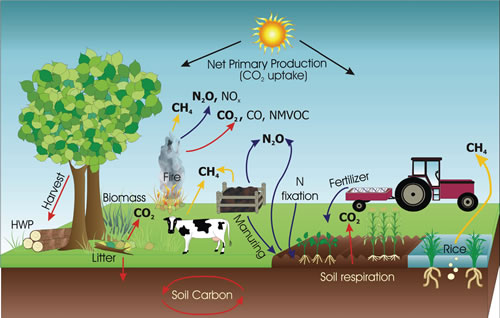
\includegraphics[width=\textwidth]{../foto/carbonCycle.jpg}
      \end{figure}}
    \only<6>{
      % \vspace{1.5cm}
      \begin{figure}[h]
        \centering
        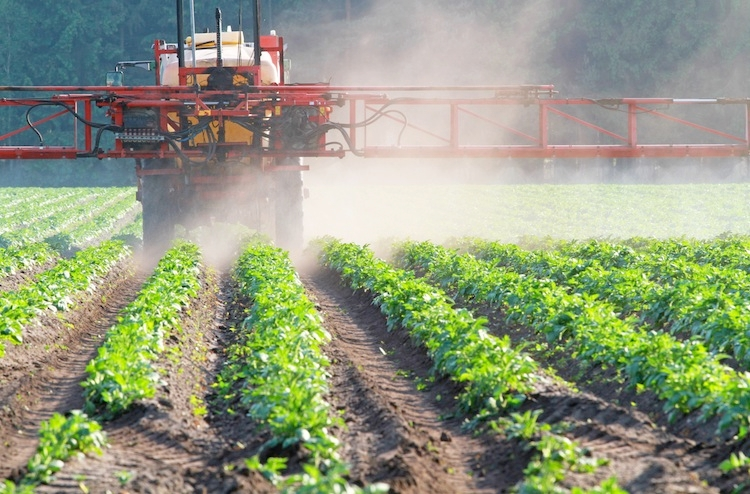
\includegraphics[width=\textwidth]{../foto/fitofarmaci.jpg}
      \end{figure}}
    \only<7>{
      % \vspace{1.5cm}
      \begin{figure}[h]
        \centering
        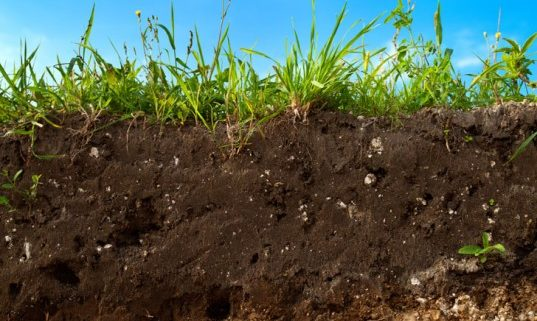
\includegraphics[width=\textwidth]{../foto/fertilitsuolo.jpg}
      \end{figure}}
  \end{columns}
\end{frame}



\begin{frame}{Parte 1 \small{Indici di fertilità}}
  Per valutare l'effetto dell'agricoltura biologica sulla fertilità
  vengono comunemente utilizzati indici:
  \begin{itemize}[<+->]
    \pause
  \item chimici
  \item biologici
  \item ecologici
  \item produttivi
  \item \Large{fisici} \onslide<7->{\Large{$\rightarrow$ trascurati
        dalla letteratura}}
    \pause
    \begin{enumerate}[<+->]
    \item Densità apparente
    \item Stabilità di struttura
    \item Distribuzione dei pori
    \end{enumerate}
  \end{itemize}
  
\end{frame}



\begin{frame}{Parte 1 \small{Obiettivi}}
  Tramite l'uso di indici di fertilità del suolo, verificare la
  presenza di differenze tra:
  \begin{columns}[c]
    \column{.50\textwidth}
    \begin{itemize}[<+->]
      \pause
    \item Metodo di conduzione (convenzionale, biologico) 

    \item Lavorazioni primarie (aratura, frangizollatura, rippatura)
    \end{itemize}
    \column{.48\textwidth}
    \only<2>{\includegraphics[width=0.8\textwidth]{../foto/logo-Bio.png}}
    \only<3>{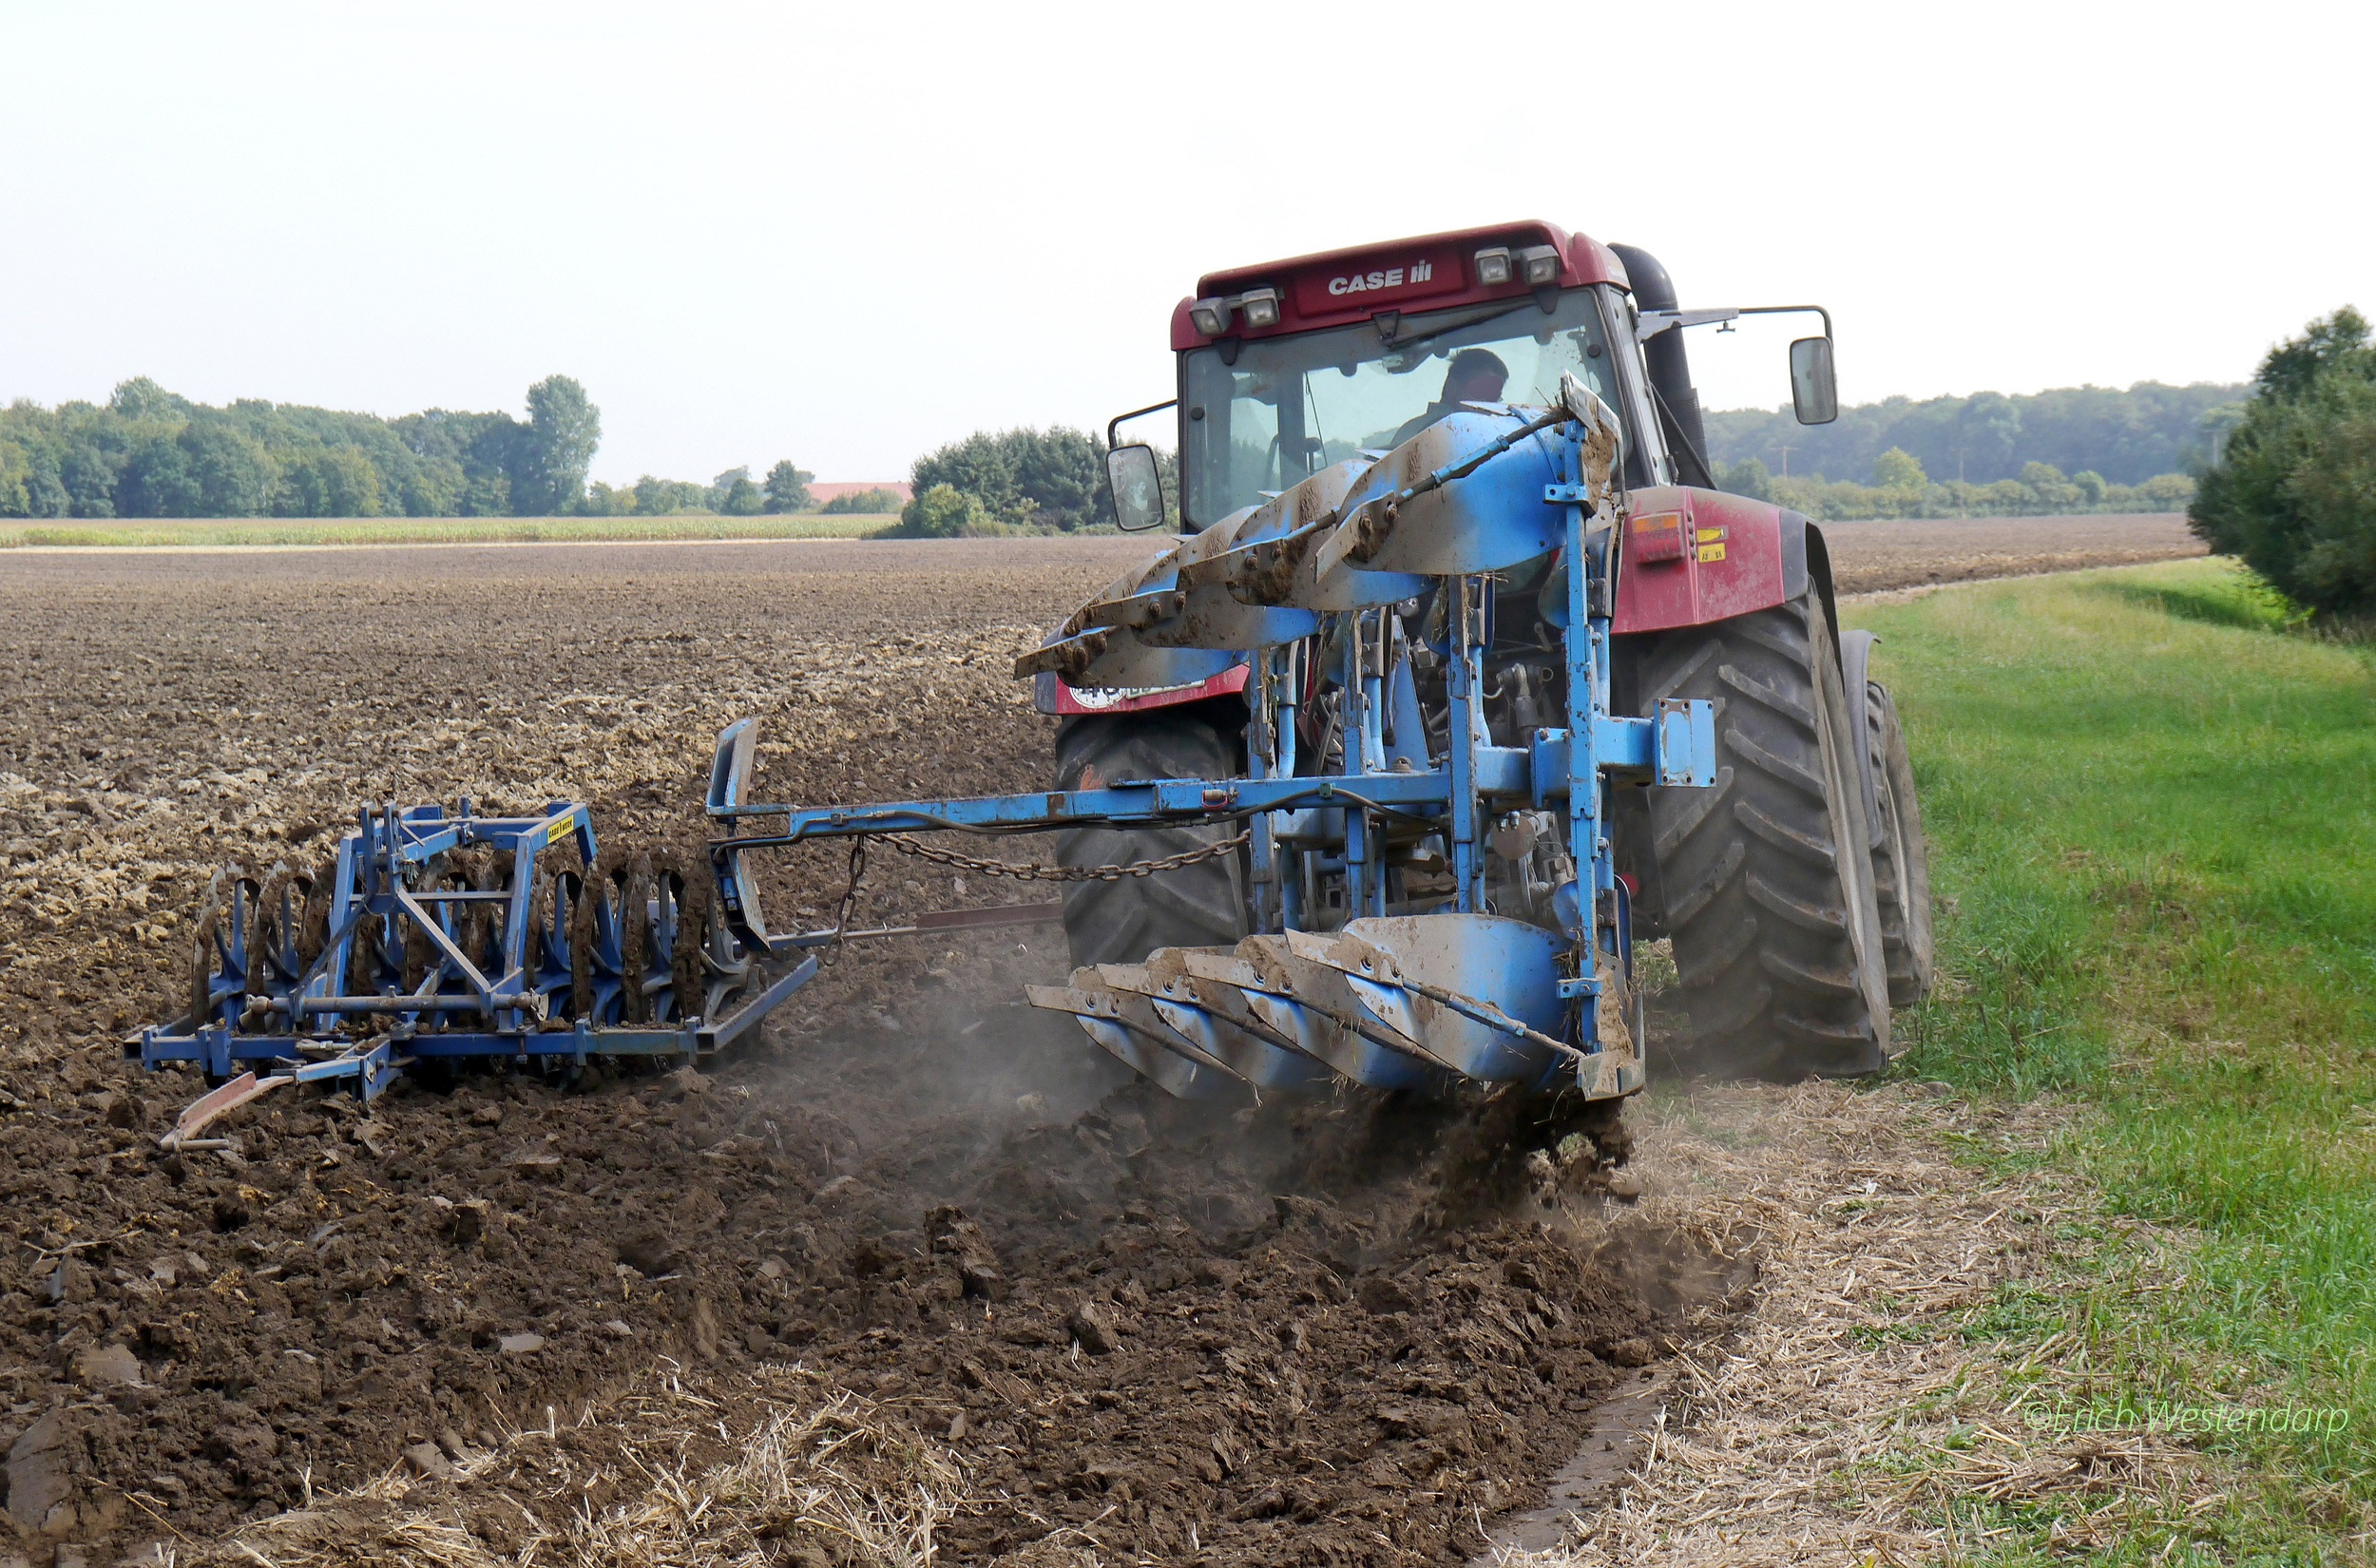
\includegraphics[width=0.8\textwidth]{../foto/lavorazione.jpg}}
  \end{columns}
\end{frame}

\begin{frame}{Parte 2 \small{Sito sperimentale}}
  \begin{minipage}[0.45\textheight]{\textwidth}
    \begin{itemize}[<+->]
    \item esperimento a lungo termine dal 1991 (MoLTE) presso Azienda
      agricola Montepaldi
    \item superficie leggermente declive di circa 15 ha a 90
      m s.l.m.
    \item area Mediterranea $\rightarrow$ ridotto apporto di concimi
      organici di origine animale
    \end{itemize}
  \end{minipage}
  \vfill
  \begin{minipage}[0.45\textheight]{\textwidth}
    \only<1>{
      \begin{figure}
        \centering
        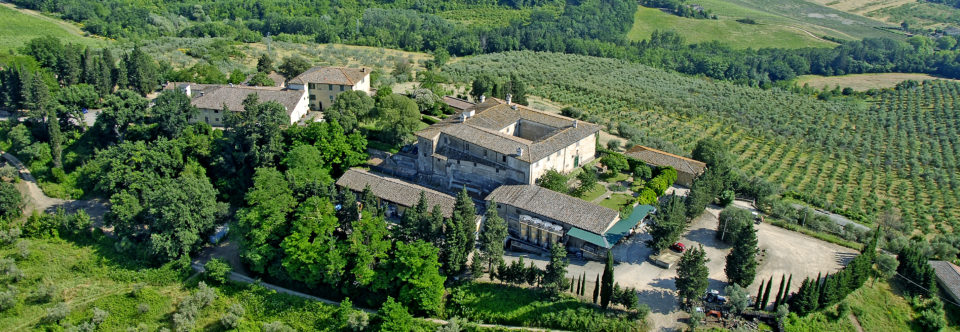
\includegraphics[width=0.9\textwidth]{../foto/Montepaldi.jpg}
      \end{figure}}

    \only<2-3>{
      \begin{figure}
        \centering
        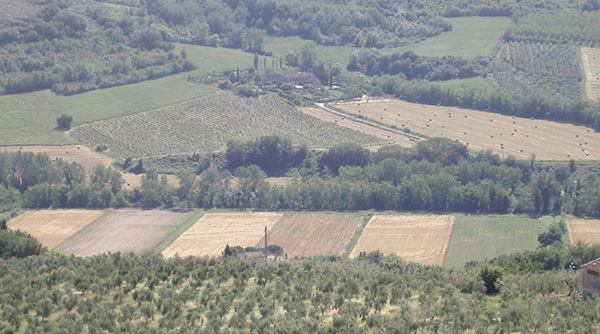
\includegraphics[width=0.7\textwidth]{../foto/campi2.jpg}
      \end{figure}}
  \end{minipage}
\end{frame}

\begin{frame}{Parte 2 \small{Sito sperimentale}}
  \begin{itemize}[<+->]
  \item 4 appezzamenti, 2 Convenzionali e 2 Biologici
  \item 9 parcelle entro appezzamento $\rightarrow$ lavorazioni con 3 repliche
  \item in ogni parcella $\rightarrow$ tre punti,
    sovracampionamento per ragioni cautelative
  \end{itemize}
  \vfill
  \only<1>{
    \begin{figure}
      \centering
      \includegraphics[width=0.6\textwidth]{../foto/bionuovovecchio.png}
    \end{figure}}
  \only<2>{
    \begin{figure}
      \centering
      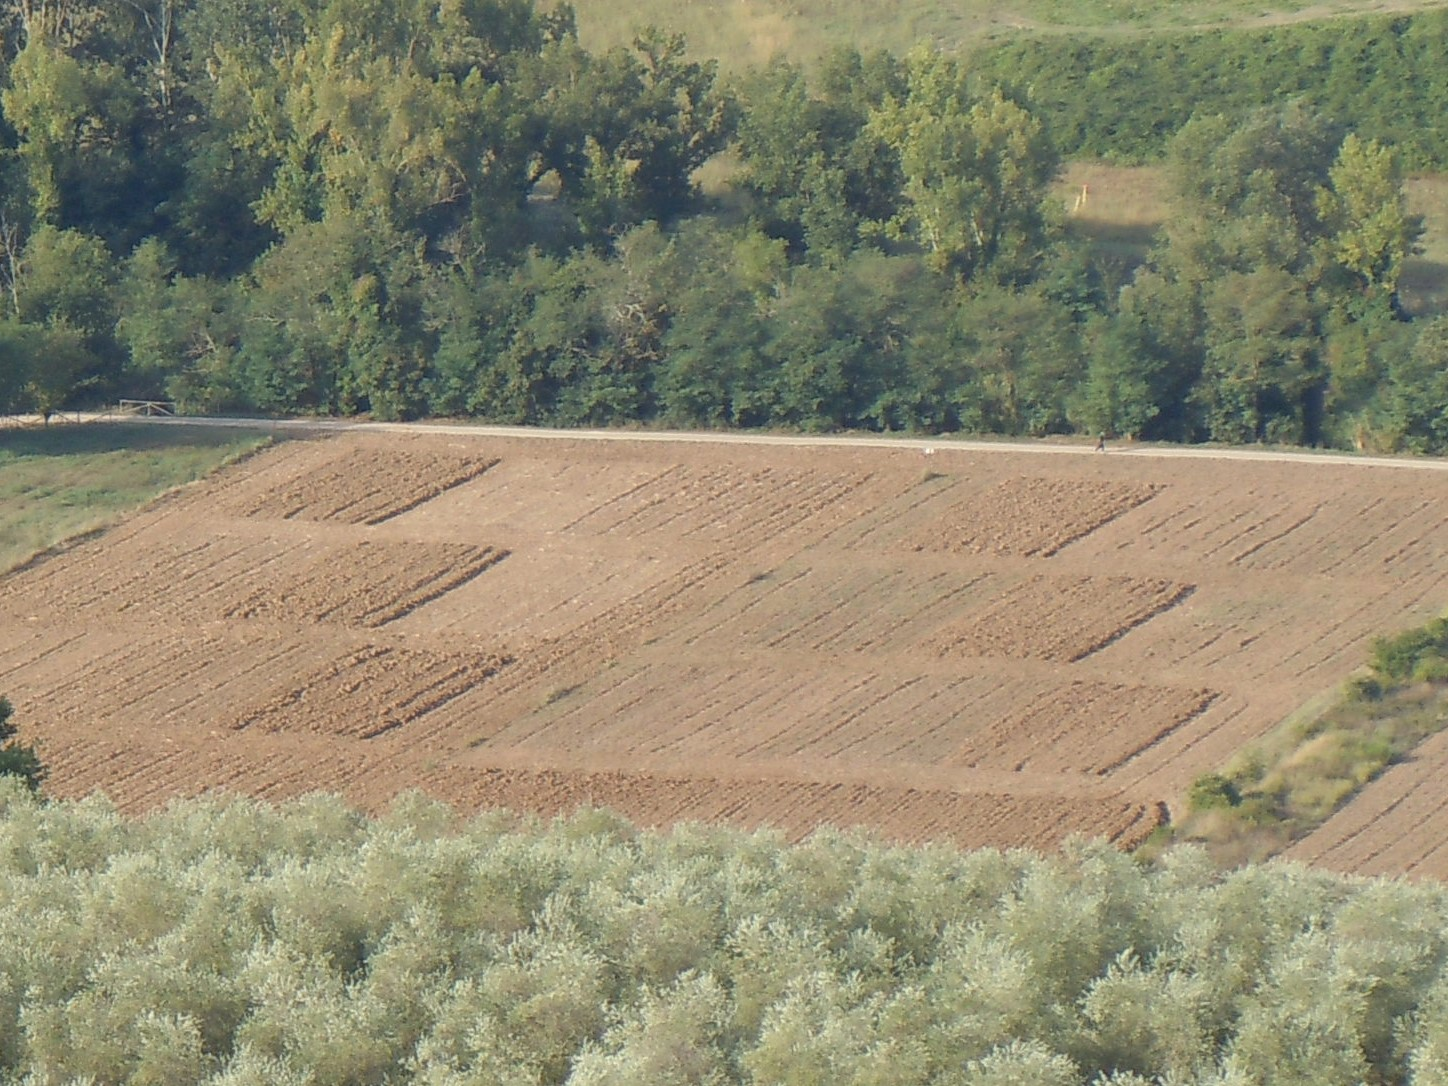
\includegraphics[width=0.5\textwidth]{../foto/Panoramica_lavorazioni.jpeg}
    \end{figure}}
  \only<3>{
  \scriptsize
  \begin{table}[ht]
    \centering
    \begin{tabular}{|l|c|c|c|}
      \hline
      Campi        & Convenzionale & Biologico   &    \\

      \hline
                   &                &                      &      \\ 
      Appezzamenti & 2              &  2                   &       \\ 

                   &                &                      &        \\
      \hline
                   &                &                      &         \\
      Parcelle     &               &                       &   \\
      entro appezzamento   &      9 &     9                &       \\

                   &                &                      &        \\
      \hline
                   &                &                      &        \\
      Punti entro  &          3     &    3                 &\\ 
      parcella     &                &                      &
      \\
      \hline
                   &                &                      &        \\
      Totale campioni& 54           &     54               &108   \\
\hline
    \end{tabular}
  \end{table}
    % \begin{figure}
    %   \centering
    %   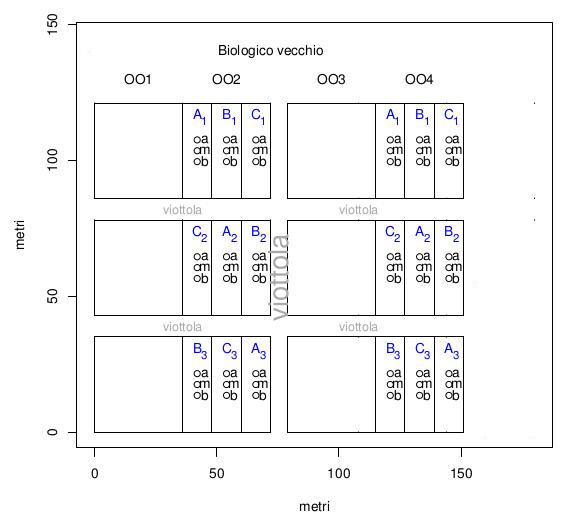
\includegraphics[width=0.5\textwidth]{../foto/OO_sito.jpeg}
    % \end{figure}
  }
\end{frame}

\begin{frame}

\end{frame}




\end{frame}

\begin{frame}{Parte 2 \small{Metodi di analisi}}
  \begin{columns}[c]
    \column{.50\textwidth}
    \begin{enumerate}[<+->]
    \item Densit\`a apparente
      \begin{itemize}
      \item Metodo Cilindro ($\sim 1000 cm^3$)
        \pause
      \item Metodo Spinta idrostatica ($\sim 30 cm^3$)
        \pause
      \end{itemize}
    \item Stabilit\`a degli aggregati tramite dinamica della
      distribuzione della dimensione degli aggregati
    \item Distribuzione dimensionale dei pori tramite tecniche di
      porosimetria ad intrusione di mercurio      
    \end{enumerate}
    \column{.48\textwidth}
    % \begin{overlayarea}{\linewidth}{3cm}
    \only<2>{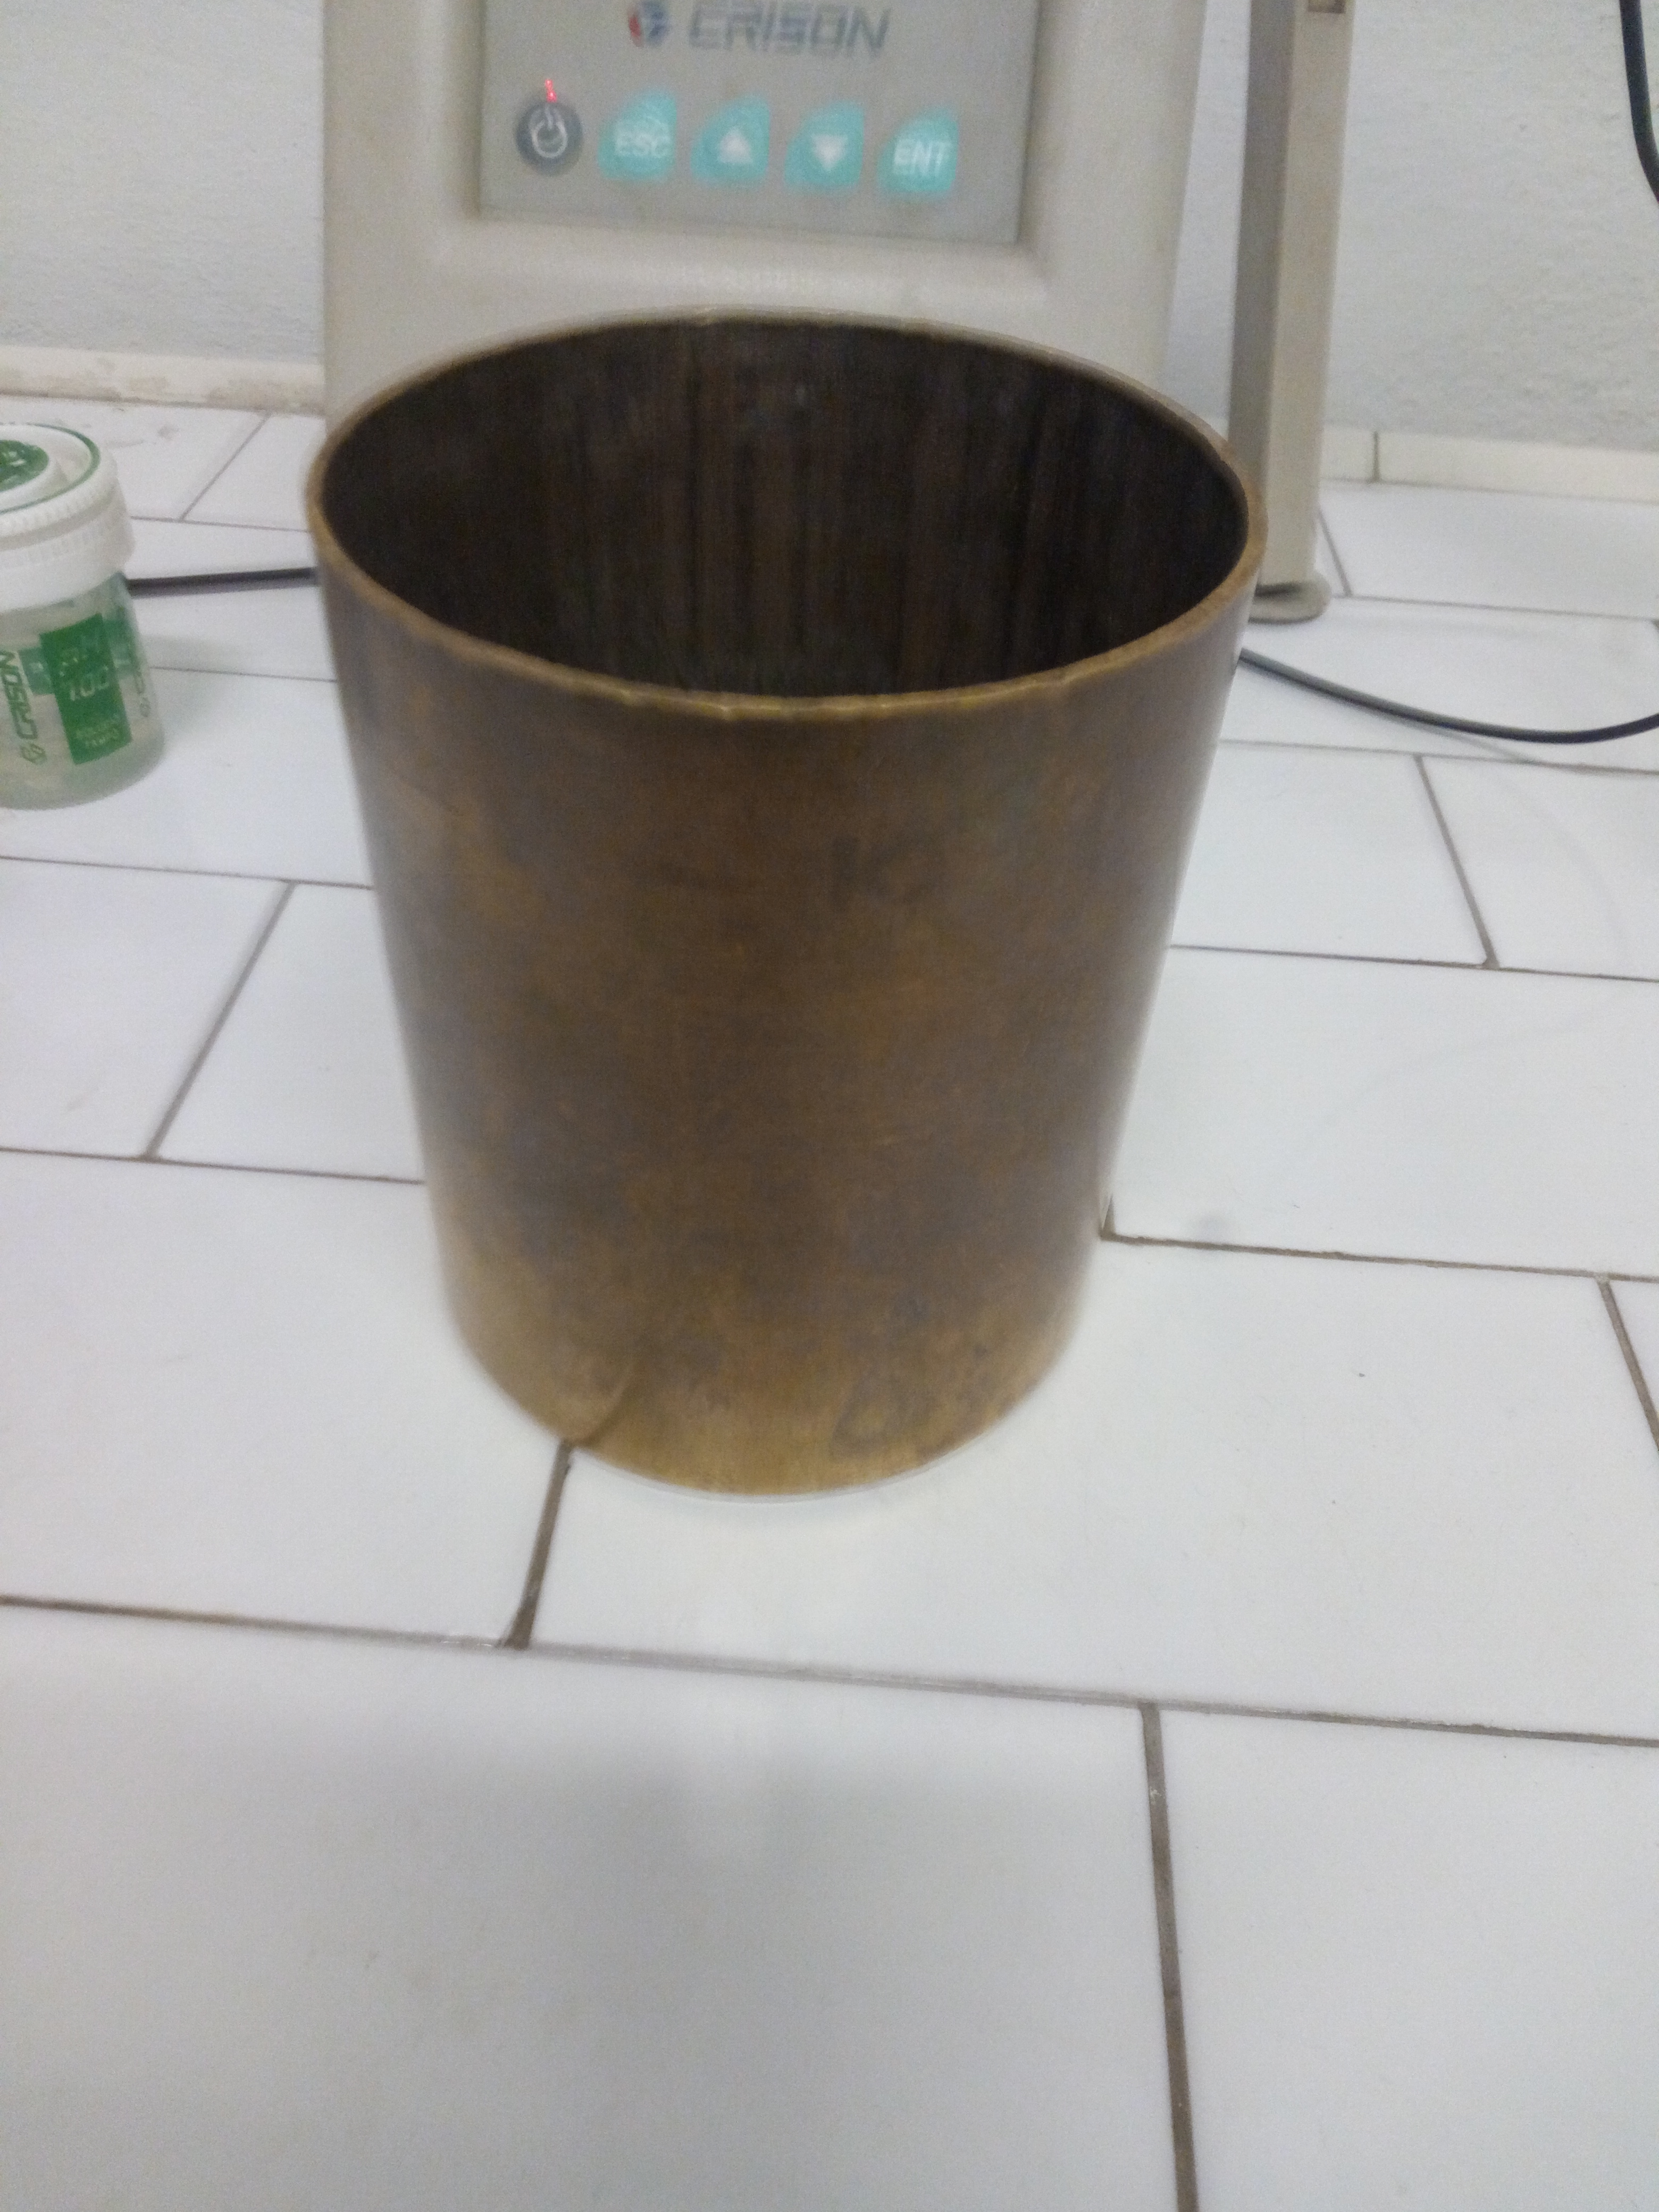
\includegraphics[width=0.8\textwidth]{../foto/cilindroOttone.jpeg}}
    \only<3>{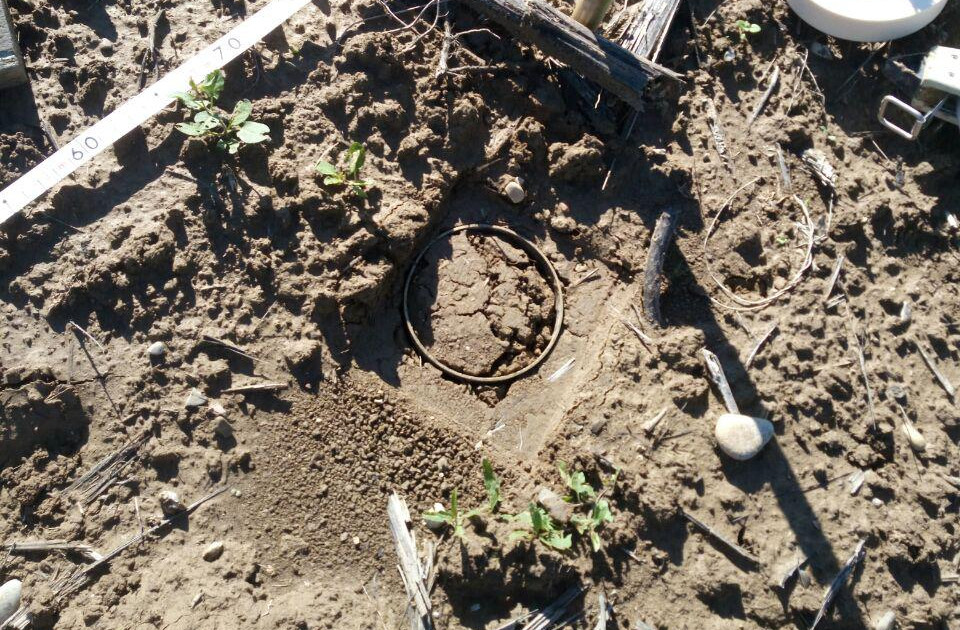
\includegraphics[width=0.8\textwidth]{../foto/cilindrosuolo.jpg}}
    \only<4>{\vspace{1cm}
      \begin{figure}[hb]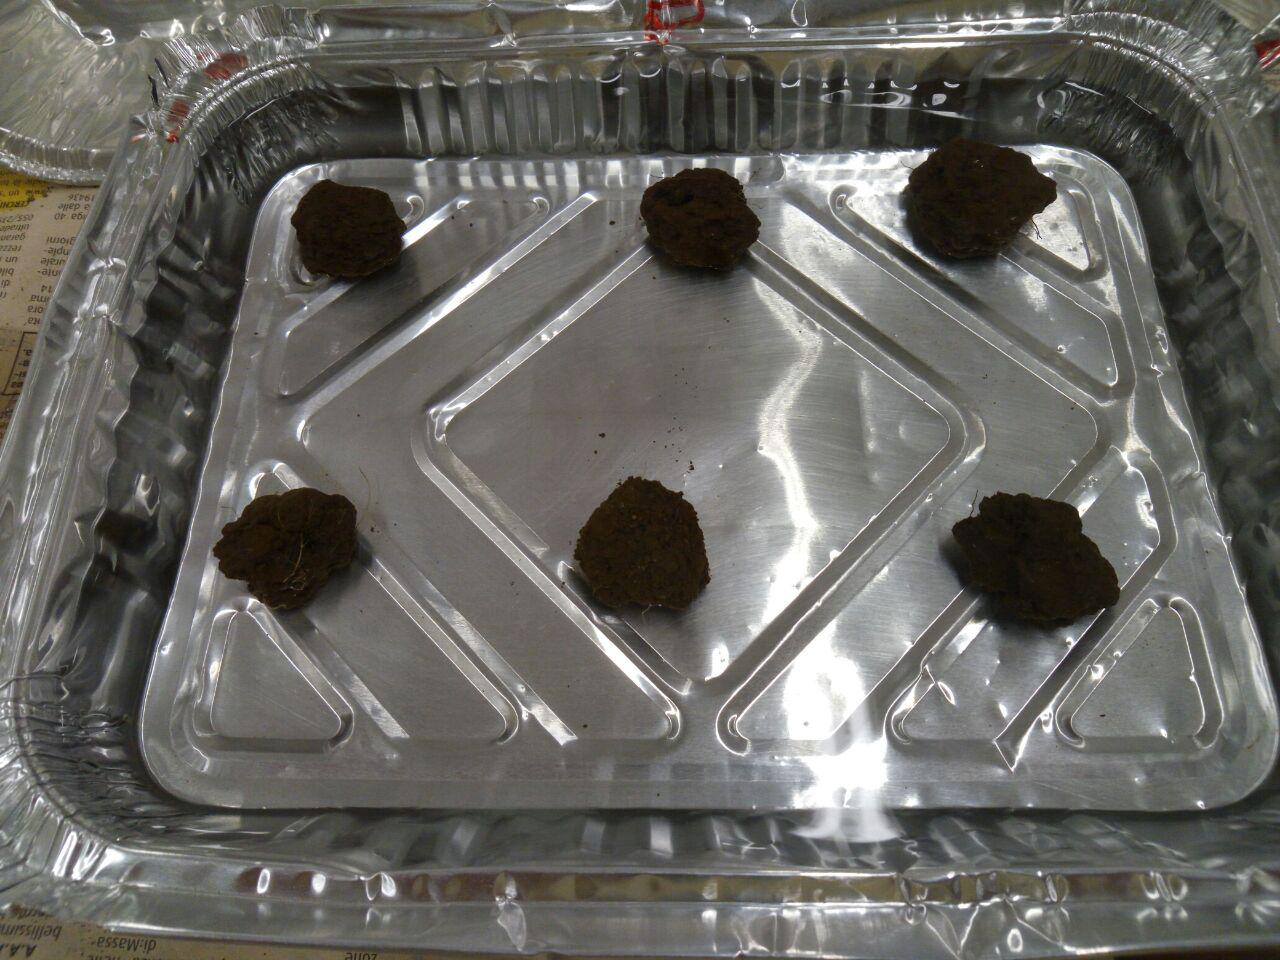
\includegraphics[width=0.8\textwidth]{../foto/petrolio}
      \end{figure}}
    \only<5>{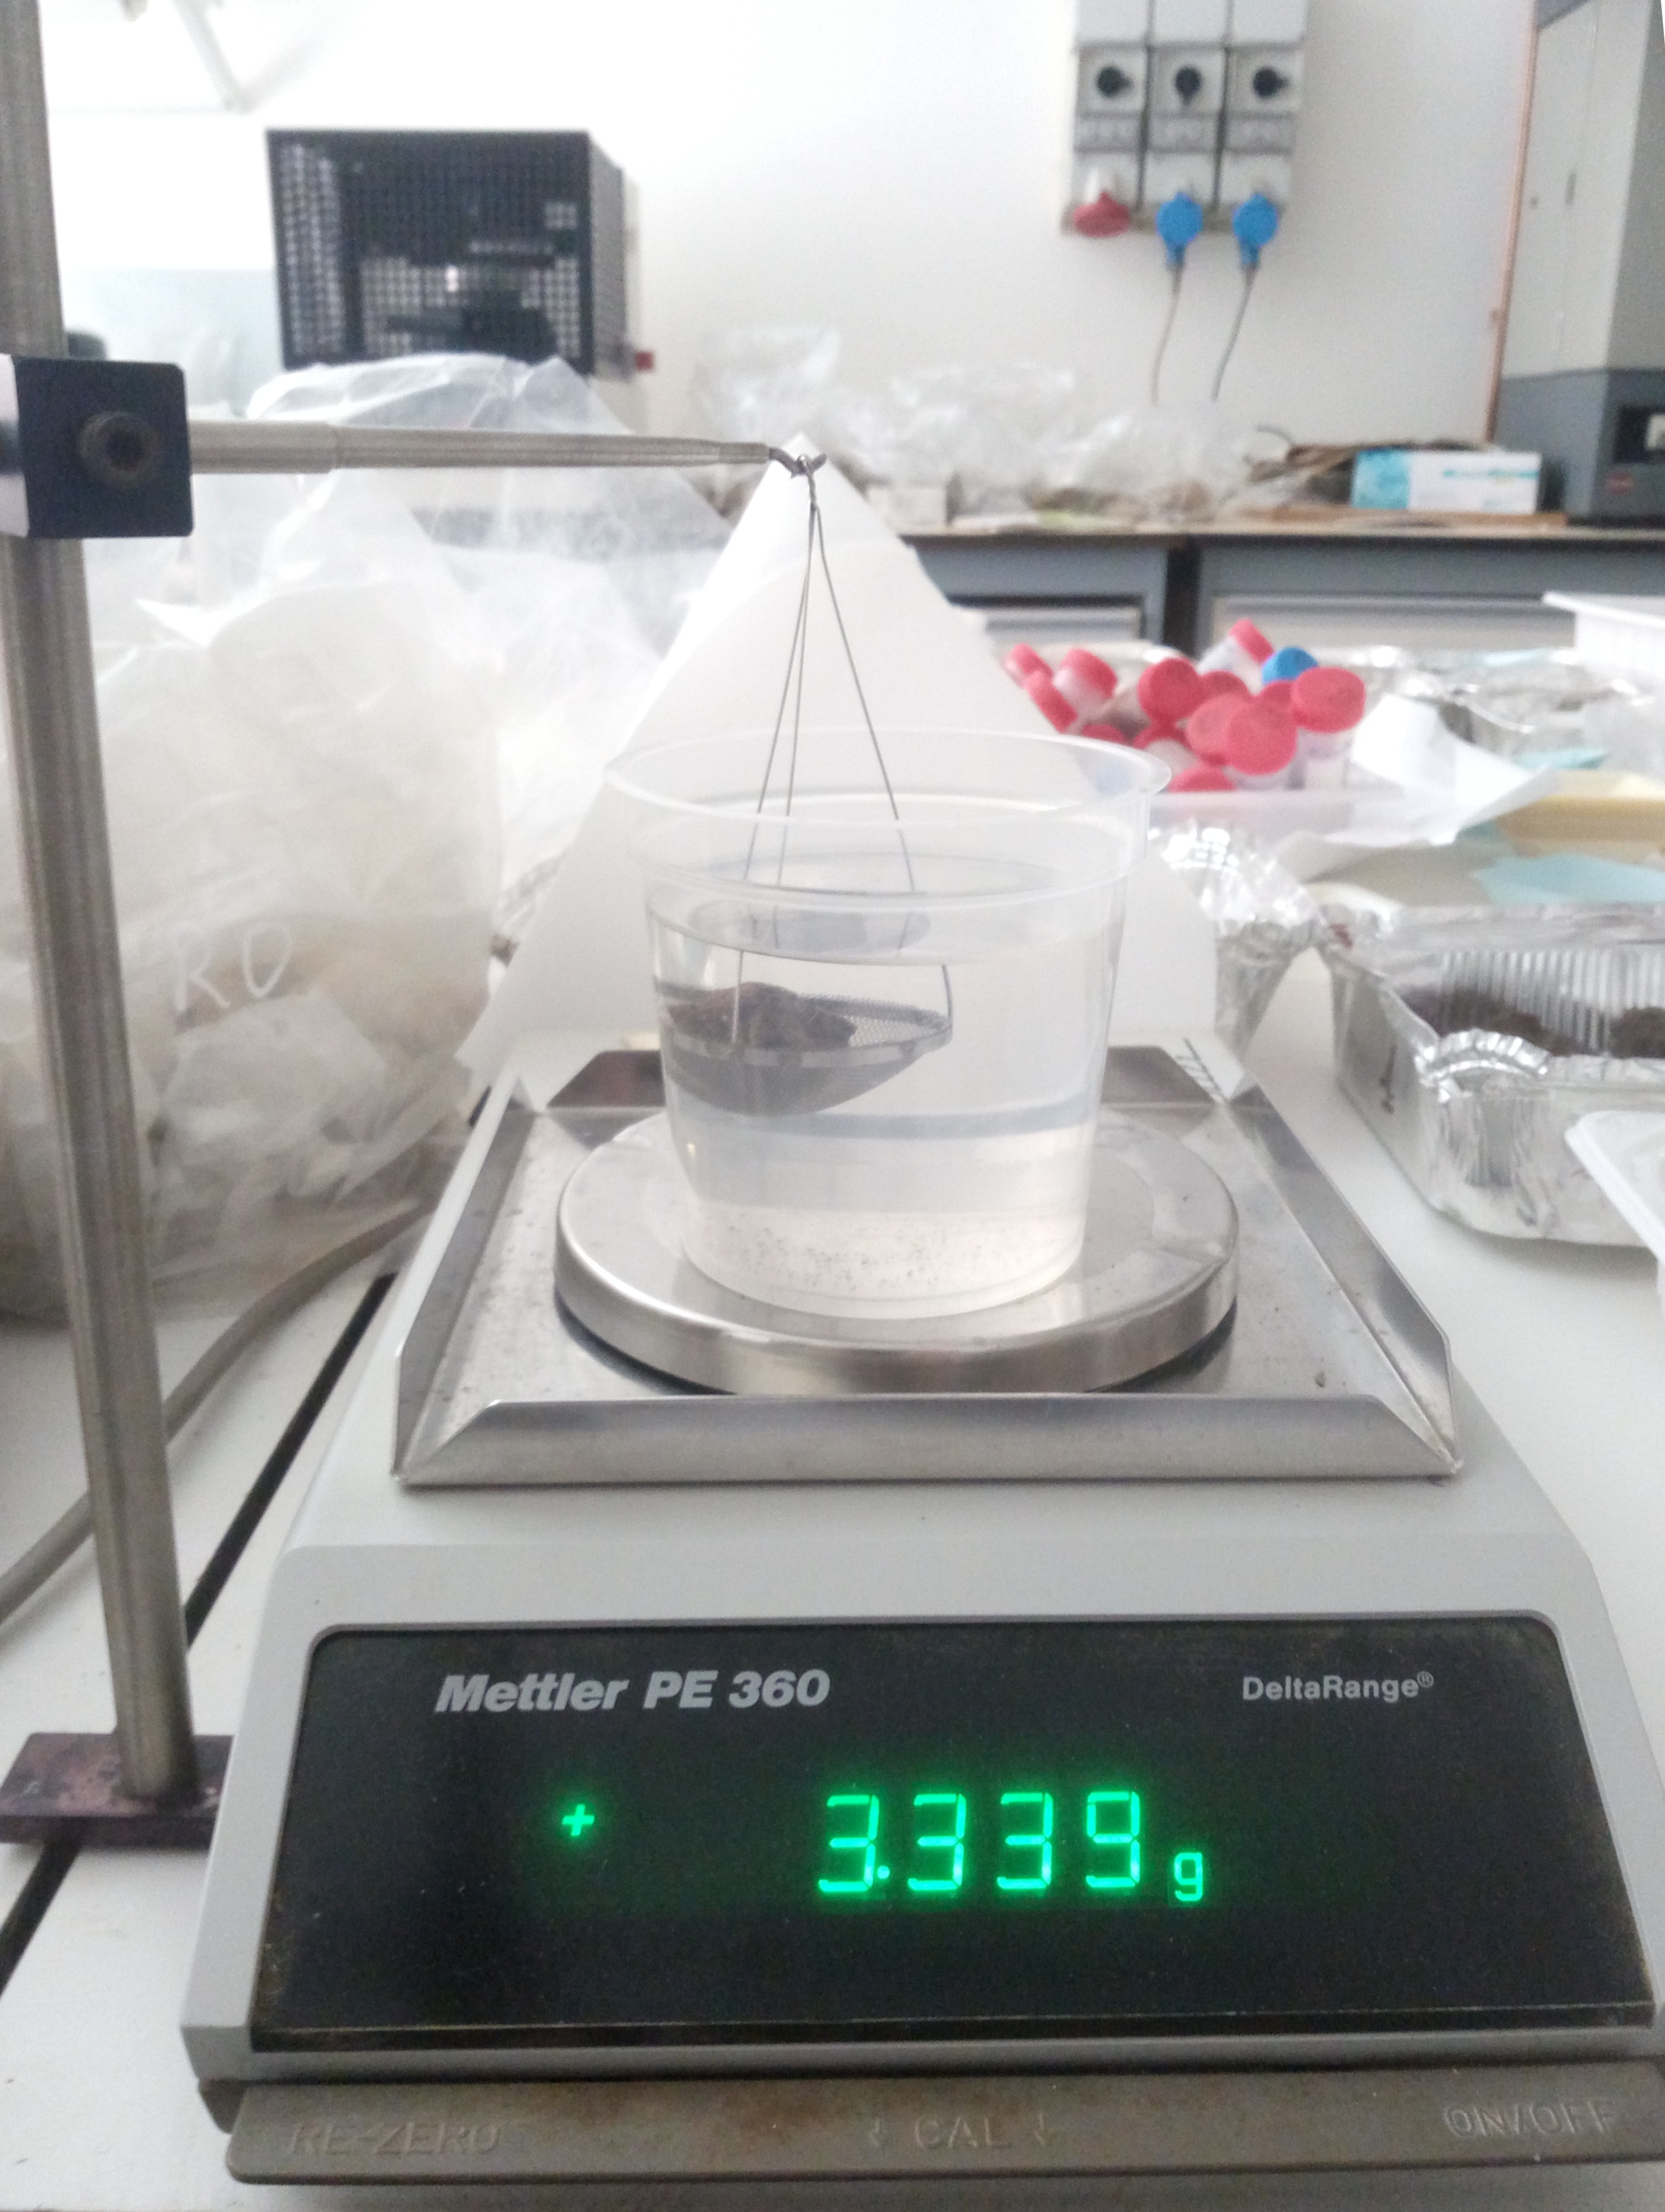
\includegraphics[width=0.8\textwidth]{../foto/navicella}}
    \only<6>{\animategraphics[loop,autoplay,width=\linewidth]{12}{../foto/msizer/Msizer-}{117}{176}
      \animategraphics[loop,autoplay,width=\linewidth]{12}{../foto/msizer/Msizer-}{208}{233}}%233
    \only<7>{\animategraphics[loop,autoplay,width=\linewidth]{12}{../foto/poresize/PoreSize-}{0}{3}}%%396
    % \end{overlayarea}
  \end{columns}
\end{frame}



\begin{frame}{Parte 2 \small{Elaborazione dei dati}}
  \transwipe<4>[direction=90]
  \begin{minipage}[0.2\textheight]{\textwidth}
    \begin{columns}[T]
      \begin{column}{0.8\textwidth}
        L'elaborazione dei dati è stata effettuata mediante il linguaggio di
        programmazione R, ed ha riguardato:
        \begin{itemize}
          \onslide<2->\item l'adattamento di un modello lineare nella forma:
          \vspace{0.25cm}
          $Y \sim \beta_0 + \beta_1x_1 + \beta_2x_2 + \epsilon$

          \onslide<3->{in cui le variabili categoriche sono:}
          \begin{itemize}

            \onslide<4->\item $\x_1$ conduzione \newline
            \emph{Convenzionale}, \emph{Biologico}

            \onslide<5->\item $\x_2$ lavorazioni \newline \emph{Arato, Rippato,
              Frangizollato}

            \onslide<6->\item$\epsilon$ residui o errore
          \end{itemize}
        \end{itemize}
      \end{column}
      \begin{column}{0.2\textwidth}
        \includegraphics[width=2.5cm]{../foto/logo-R.png}
      \end{column}
    \end{columns}
  \end{minipage}

  \begin{itemize}
    \onslide<7->\item la validazione del modello attraverso l'analisi
    dei residui 
    \onslide<8->\item verifica della significatività delle
    ipotesi mediante analisi della varianza (ANOVA)
  \end{itemize}
\end{frame}


% \begin{frame}[label=Composizionale]
%   \vspace{2cm}
%   Risultati analisi \hyperlink{Anova}{\beamerbutton{composizionale}}
%   \begin{figure}[hb]
%     \includegraphics[width=0.6\textwidth]{../tesi/Tesi_GIT-plotacompWETDRY.pdf}
%   \end{figure}
% \end{frame}

\begin{frame}
  \finalpage{\Huge{Risultati}}
\end{frame}


\begin{frame}{Parte 3 \small{boxplot metodo Cilindro}}
  
  \begin{figure}
    \includegraphics[width=0.6\textwidth]{../tesi/boxCore.pdf}
  \end{figure}
\end{frame}

\begin{frame}{Parte 3 \small{ ANOVA metodo  Cilindro} }
  % latex table generated in R 3.4.0 by xtable 1.8-2 package
  % Thu Jun 22 16:16:27 2017
  \begin{table}[ht]
    \centering
    \label{tab:anova del modello}
    \begin{tabular}{lrrrrr}
      \hline
      & Df & Sum Sq & Mean Sq & F value & Pr($>$F) \\ 
      \hline 
      Anno         & 1  &  0.02  &  0.02  &   1.41   & 0.2390   \\ 
      Conduzione   & 1  &  0.04  &  0.04  &   3.29   & 0.0745   \\ 
      Lavorazione  & 2  &  0.00  &  0.00  &   0.03   & 0.9728   \\ 
      Residui      & 90 &  0.97  &  0.01  &          &          \\ 
      \hline
    \end{tabular}
  \end{table}
\end{frame}

\begin{frame}[label=Clod]{Parte 3 \small{ metodo Spinta idrostatica}}
  \hyperlink{finale}{\beamerbutton{Conclusioni}}
  \footnotesize
  \begin{table}[ht]
    \centering
    \begin{tabular}{llrccc}
      \hline
      Conduzione    & Lavorazione   & Media& Dev. std & n    & Tukey \\ 
      \hline
      Convenzionale & Arato         & 1.93 & 0.06      &  18 & b     \\ 
                    & Frangizollato & 1.89 & 0.05      &  18 & ab    \\ 
                    & Rippato       & 1.90 & 0.06      &  18 & ab    \\ 
      Biologico     & Arato         & 1.90 & 0.07      &  18 & ab    \\ 
                    & Frangizollato & 1.84 & 0.06      &  18 & a     \\ 
                    & Rippato       & 1.87 & 0.07      &  18 & ab    \\ 
      \hline
    \end{tabular}
    \label{tab:RiassuntoDensitaSpinta}
  \end{table}
\end{frame}

\begin{frame}{Parte 3 \small{Boxplot metodo Spinta idrostatica}} 
  \begin{figure}
    \includegraphics[width=0.6\textwidth]{../tesi/boxClod.pdf}
  \end{figure}
\end{frame}


\begin{frame}{Parte 3 \small{ ANOVA metodo Spinta idrostatica}}
  % latex table generated in R 3.4.0 by xtable 1.8-2 package
  % Thu Jun 22 16:32:35 2017
  \begin{table}
    \centering
    \begin{tabular}{llcccc}
      \hline
      & Df  & Sum Sq & Mean Sq & F value & Pr($>$F) \\ 
      \hline
      Conduzione  & 1   & 0.03   & 0.03    & 6.31    & 0.012    \\ 
      Lavorazione & 2   & 0.05   & 0.02    & 5.83    & 0.004    \\ 
      Totale      & 104 & 0.42   & 0.00    &         &          \\ 
      \hline
    \end{tabular}
    \label{tab:Anova densita per spinta}
  \end{table}
\end{frame}


% \begin{frame}{Parte 3 \small{Dati composizionali}}

%   \begin{columns}
%     \column{.50\textwidth}
%     \vspace{1cm}
%     \footnotesize
%     \begin{itemize}[<+->]
%     \item Dati ottenuti dalle analisi di porosimetria e
%       stabilità degli aggregati $\rightarrow$ \emph{dati Composizionali}%sono delle distribuzioni in cui ogni
%       %       classe dimensionale è espressa come percentuale sul volume totale,
%       %       questo tipo di dati prende il nome di
%       \pause
%     \item Per rappresentare i dati composizionali si utilizza un
%       grafico triangolare. Per l'elaborazione è necessaria
%       un'operazione di linearizzazione
%     \item Operazioni sono state effettuate tramite il package 'composition'
%     \end{itemize}

%     \column{.48\textwidth}
%     \only<2>{\begin{overlayarea}{\linewidth}{3cm}
%       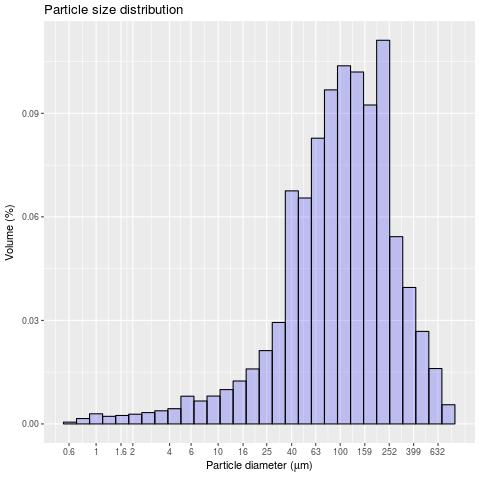
\includegraphics[width=\textwidth]{../grafici/boh.jpeg}
%     \end{overlayarea}}
%     \only<3>{\includegraphics[width=0.5\textwidth]{../foto/simplessodeformaVerticale.png}}
%     \only<4>{\includegraphics[width=\textwidth]{../tesi/Tesi_GIT-figboh.pdf}}
%   \end{columns}
% \end{frame}





\begin{frame}[label=distribuzione]{Parte 3 \small{Diagramma ternario Stabilità}}
  \hyperlink{finale}{\beamerbutton{Conclusioni}}
  
  \begin{figure}
    \includegraphics[width=0.6\textwidth]{../tesi/Tesi_GIT-figboh.pdf}
  \end{figure}
\end{frame}



\begin{frame}[label=Anova]{Parte 3 \small{Anova Stabilità}}
  \hyperlink{Composizionale}{\beamerbutton{Conclusioni}}
  \footnotesize
  % latex table generated in R 3.4.0 by xtable 1.8-2 package
  % Tue Jun 27 21:29:19 2017
  \begin{table}
    \centering
    \begin{tabular}{lrrrrcr}
      \hline
      & Df&Pillai& approx F & num Df & den Df & Pr($>$F) \\ 
      \hline
      Convenzionale & 1 & 0.92 & 4955.26  &      2 &    835 & $<10^{-3}$\\ 
      Biologico     & 1 & 0.09 & 41.72    &      2 &    835 & $<10^{-3}$\\ 
      Tempo         & 1 & 0.92 & 4504.77  &      2 &    835 & $<10^{-3}$\\ 
      Tempo$^2$     & 1 & 0.35 & 227.06   &      2 &    835 & $<10^{-3}$\\ 
      Totale        & 836 &    &          &        &        &          \\ 
      \hline
    \end{tabular}
  \end{table}
\end{frame}

\begin{frame}[label=Porosimetria]{Parte 3 \small{Porosimetria}}
  \hyperlink{finale}{\beamerbutton{Conclusioni}}
  
  \begin{figure}
    \includegraphics[width=0.6\textwidth]{../tesi/Tesi_GIT-figurina.pdf}
  \end{figure}
\end{frame}

\begin{frame}{Parte 3 \small{Sommario Porosimetria}}

  \footnotesize
  \begin{table}[hb]
    \centering
    % \caption{Distribuzione dei pori nelle tre classi dimensionali dei dati ottenuti dalla analisi 
    % con porosimetria a mercurio} 
    % \label{tab:Poro_medie}
    \begin{tabular}{llccc}%p{1.25cm}p{3.25cm}p{2cm}}
      \hline
      Conduzione & Lavorazione & Residui & Immagazzinamento &
                                                              Trasmissione \\ 
                 &             & (\%) &  (\%) &  (\%) \\ 
      \hline
      Convenzionale & Arato & 74 & 24 & 2 \\ 
                 & Rippato & 61 & 34 & 6 \\ 
                 & Frangizollato & 65 & 33 & 2 \\ 
                 &  &  &  &  \\ 
      Biologico & Arato & 56 & 41 & 3 \\ 
                 & Rippato & 56 & 41 & 3 \\ 
                 & Frangizollato & 64 & 32 & 4 \\ 
      \hline
    \end{tabular}
  \end{table}
\end{frame}

\begin{frame}{Parte 3 \small{Anova Porosimetria}}
  \begin{table}[ht]
    \centering
    % \caption{Analisi della varianza relativa al modello composizionale dei dati ottenuti dalle analisi con porosimetria a mercurio } 
    % \label{tab:poros_anova}
    \begin{tabular}{lrrrrrr}
      \hline
      & Df & Pillai & approx F & num Df & den Df & Pr($>$F) \\ 
      \hline
      Intercetta & 1 & 0.94 & 60.45 & 2 & 7 & $<10^{-3}$ \\ 
      Conduzione & 1 & 0.14 & 0.58 & 2 & 7 & 0.585 \\ 
      Lavorazione & 2 & 0.52 & 1.41 & 4 & 16 & 0.275 \\ 
      Totale & 8 &  &  &  &  &  \\ 
      \hline
    \end{tabular}
  \end{table}
\end{frame}


\begin{frame}[label=finale]{Parte 4 \small{Conclusioni}}
  \begin{enumerate}[<+->]

  \item densità apparente:
    \begin{itemize}
    \item metodo \hyperlink{Core}{\beamerbutton{Core}}, nonostante la semplicità esecutiva,
      sembra inadeguato a cogliere differenze di qualsiasi genere
      (\emph{anno, lavorazione, conduzione}).
    \item metodo \hyperlink{Clod}{\beamerbutton{Clod}} mostra differenze significative, ma di
      una entità tale da non risultare tecnologicamente rilevanti.
    \end{itemize}
  \item \hyperlink{distribuzione}{\beamerbutton{distribuzione}} dinamica: riscontrata una
    maggiore stabilità degli aggregati provenienti da appezzamenti
    \emph{Convenzionali} rispetto a quelli provenienti da appezzamenti
    \emph{Biologici}; non sono state riscontrate differenze significative
    all'interno trattamenti di \emph{lavorazione}.
  \item \hyperlink{Porosimetria}{\beamerbutton{porosimetria}}: tendenza da parte dei suoli
    \emph{Biologici} ad essere più porosi e con pori mediamente più
    grandi dei campioni di suolo \emph{Convenzionali}.
  \end{enumerate}

\end{frame}

\begin{frame}{Parte 4 \small{Aspetti produttivi}}

  \vspace{0.5cm}
  \footnotesize{
    \begin{table}[ht]
      \centering
      \begin{tabular}{lllcc}
        \hline
        Conduzione   & Anno & Lavorazione   & Orzo(t/ha)      & Girasole(t/ha) \\ 
        \hline
        Biologico    & 2016 & Arato         & 3.7 $\pm$ 0.04  & 2.5 $\pm$ 0.75 \\ 
                     &      & Rippato       & 3.3 $\pm$ 0.25  & 2.9 $\pm$ 0.47 \\ 
                     &      & Frangizollato & 3.2 $\pm$ 0.08  & 1.6 $\pm$ 0.05 \\ 
                     & 2017 & Arato         & 2.9 $\pm$ 0.08  & 1.4 $\pm$ 0.33 \\ 
                     &      & Rippato       & 2.3 $\pm$ 0.27  & 1.0 $\pm$ 0.10 \\ 
                     &      & Frangizollato & 2.2 $\pm$ 0.17  & 1.1 $\pm$ 0.18 \\ 
        Convenzionale& 2016 & Arato         & 5.0 $\pm$ 0.16  & 4.5 $\pm$ 0.38 \\ 
                     &      & Rippato       & 5.0 $\pm$ 0.23  & 3.4 $\pm$ 0.08 \\ 
                     &      & Frangizollato & 5.0 $\pm$ 0.20  & 2.7 $\pm$ 0.07 \\ 
                     & 2017 & Arato         & 4.5 $\pm$ 0.19  & 0.2 $\pm$ 0.18 \\ 
                     &      & Rippato       & 4.5 $\pm$ 0.11  & 0.2 $\pm$ 0.27 \\ 
                     &      & Frangizollato & 3.9 $\pm$ 0.21  & 0.4 $\pm$ 0.18 \\ 
        \hline
      \end{tabular}
    \end{table}}



\end{frame}



\begin{frame}
  \finalpage{Grazie per l'attenzione.}
\end{frame}

%%% Local Variables:
%%% mode: latex
%%% TeX-master: t
%%% End:
\appendix
% \section{More}
% \begin{frame}[label=supplemental]
%   Supplemental content.
%   Back to .
% \end{frame}

% \subsection{Risultati Core}

\end{document}

%%% Local Variables:
%%% mode: latex
%%% TeX-master: t
%%% End:
